\begin{figure}
	\begin{subfigure}{\linewidth}
		\centering
		\begin{adjustbox}{width=.8\textwidth}
			\begin{tikzpicture}
				\node[inner sep=0pt, xshift=50, yshift=-50] (shiftedcat) {
					{\transparent{.5}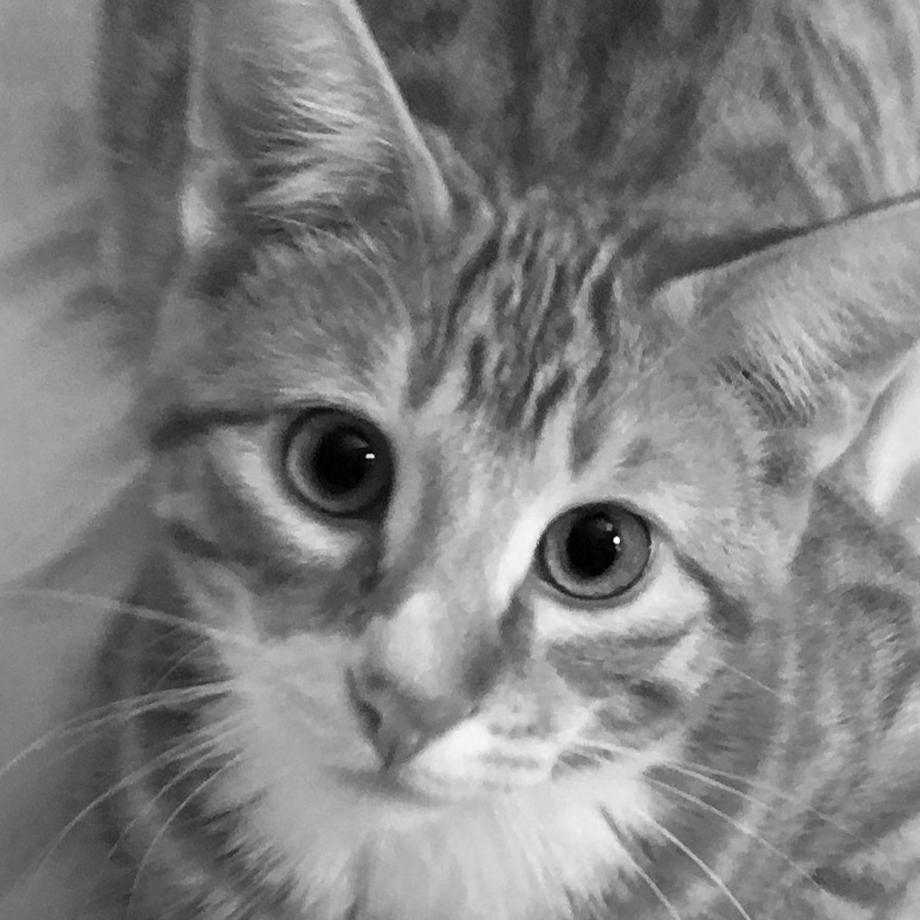
\includegraphics[]
							{figures/registration/cross-correlation/trimmed_cat.jpg}
						}};
				\node[inner sep=0pt, xshift=-50pt, yshift=50pt] (shiftedcat) {
					{\transparent{0.5}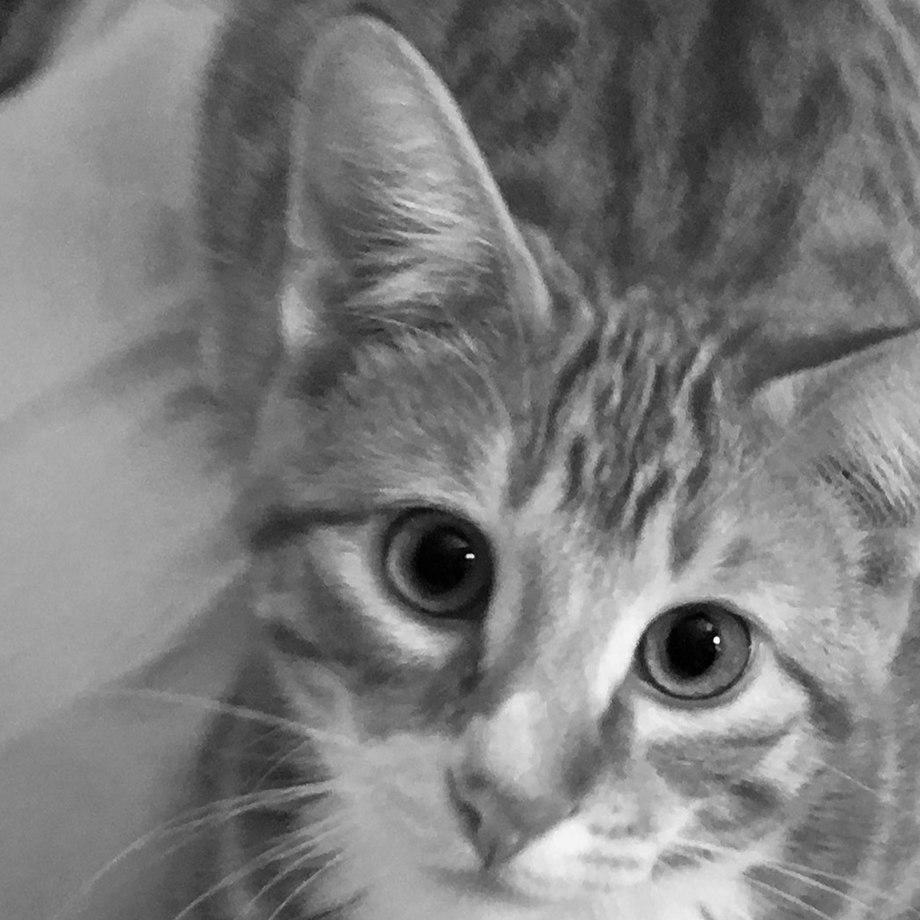
\includegraphics[]
							{figures/registration/cross-correlation/shifted_trimmed_cat.jpg}
						}};
				\draw[red, line width=1mm] (-250pt,-250pt) rectangle (250pt,250pt);
				\node(corrwin) at (0,250pt) {};
				\node[label={[label distance=1cm]:\scalebox{5}{Fixed cross-correlation window}}] (corrw) at (0,600pt) {};
				\draw[redarrow, line width=1mm] (corrw)--(corrwin);
			\end{tikzpicture}
		\end{adjustbox}
		\caption{100 pixel shifted images.} \label{fig:shiftedcat}
	\end{subfigure}
	\vskip\baselineskip
	\begin{subfigure}{\linewidth}
		\centering
		\begin{tikzpicture}
			\begin{axis}
				\addplot3 [surf, mesh/rows=19, mesh/ordering=x varies, shader=interp]
				table[col sep=comma] {figures/registration/cross-correlation/surf.csv};
				\node[above] at (axis cs:-110,-110,224141) {$(-100, -100)$};
			\end{axis}
		\end{tikzpicture}
		\caption{Cross-correlation for various $\Delta x, \Delta y$ shifts, with highest correlation at the shift.}
		\label{fig:crosscorr}
	\end{subfigure}
	\vskip\baselineskip
	\begin{subfigure}{\linewidth}
		\centering
		\begin{tikzpicture}
			\begin{axis}
				\addplot3 [surf, mesh/rows=19, mesh/ordering=x varies, shader=interp]
				table[col sep=comma] {figures/registration/cross-correlation/delta_surf.csv};
				\node[above] at (axis cs:-110,-110,1) {$(-100, -100)$};
			\end{axis}
		\end{tikzpicture}
		\caption{Phase-correlation for various $\Delta x, \Delta y$ shifts, with single peak at the correct shift.}
		\label{fig:phasecorr}
	\end{subfigure}
	\caption{Cross-correlation feature matching.}
	\label{fig:nccshift}
\end{figure}
